\documentclass[11pt]{article}
\usepackage[a4paper,margin=22mm,headheight=16pt]{geometry}
\usepackage{fontspec,xeCJK,xcolor,graphicx,enumitem,fancyhdr,titlesec}
\usepackage{hyperref}
\IfFontExistsTF{Times New Roman}{\setmainfont{Times New Roman}}{\setmainfont{TeX Gyre Termes}}
\IfFontExistsTF{FangSong}{\setCJKmainfont[AutoFakeBold=2]{FangSong}}{\IfFontExistsTF{仿宋}{\setCJKmainfont[AutoFakeBold=2]{仿宋}}{\IfFontExistsTF{FandolFang-Regular.otf}{\setCJKmainfont[AutoFakeBold=2]{FandolFang-Regular.otf}}{\setCJKmainfont{FandolSong-Regular.otf}}}}
\definecolor{ink}{HTML}{173747}\definecolor{accent}{HTML}{227E82}
\hypersetup{colorlinks=true,urlcolor=accent,linkcolor=accent}
\linespread{1.22}\setlength{\parindent}{0pt}\setlength{\parskip}{6pt}
\setlist[itemize]{leftmargin=1.4em,itemsep=3pt}
\titleformat{\section}{\large\bfseries\color{ink}}{}{0pt}{}
\titlespacing*{\section}{0pt}{14pt}{7pt}
\pagestyle{fancy}\fancyhf{}\lhead{\small OMNI LEARNING / 学习手册}\rhead{\small Source-grounded learning}\cfoot{\small\thepage}
\emergencystretch=2em\widowpenalty=10000\clubpenalty=10000
\newcommand{\Needspace}[1]{\par\begingroup\dimen0=#1\relax\vskip0pt plus\dimen0\penalty-100\vskip0pt plus-\dimen0\vskip\dimen0\penalty9999\vskip-\dimen0\vskip0pt\endgroup}
\begin{document}


{\LARGE\bfseries\color{ink} 从聊天回答到完成任务}\par

2026-10-08 | Day01/30 | 阅读 8 分钟 + 练习 3 分钟\par\vspace{6pt}

\Needspace{5\baselineskip}\section*{今日导航}

今天回答：一个会聊天的助手，什么时候才算在完成任务？目标是写清用户目标、可观察的完成条件和行动边界。面向通用产品经理，不假设你做过某个行业。课程中的旅行助手是教学方案，不代表某厂商现成功能。

\Needspace{5\baselineskip}\section*{从一句话需求拆起}

用户说：“帮我安排下周去上海出差。”一个回答可能只给攻略；一个任务系统还可能澄清时间、查询候选行程、整理费用，并等待确认。需求原句没有自动授权购买，也没有提供预算、证件或差旅政策。产品设计先补齐任务边界，再决定哪些部分交给模型。

图 A 的卡片代表目标，候选方案代表中间产物。把候选生成与最终购买区分开，就能避免用“输出了漂亮文字”代替“用户事情办成了”。

\begin{center}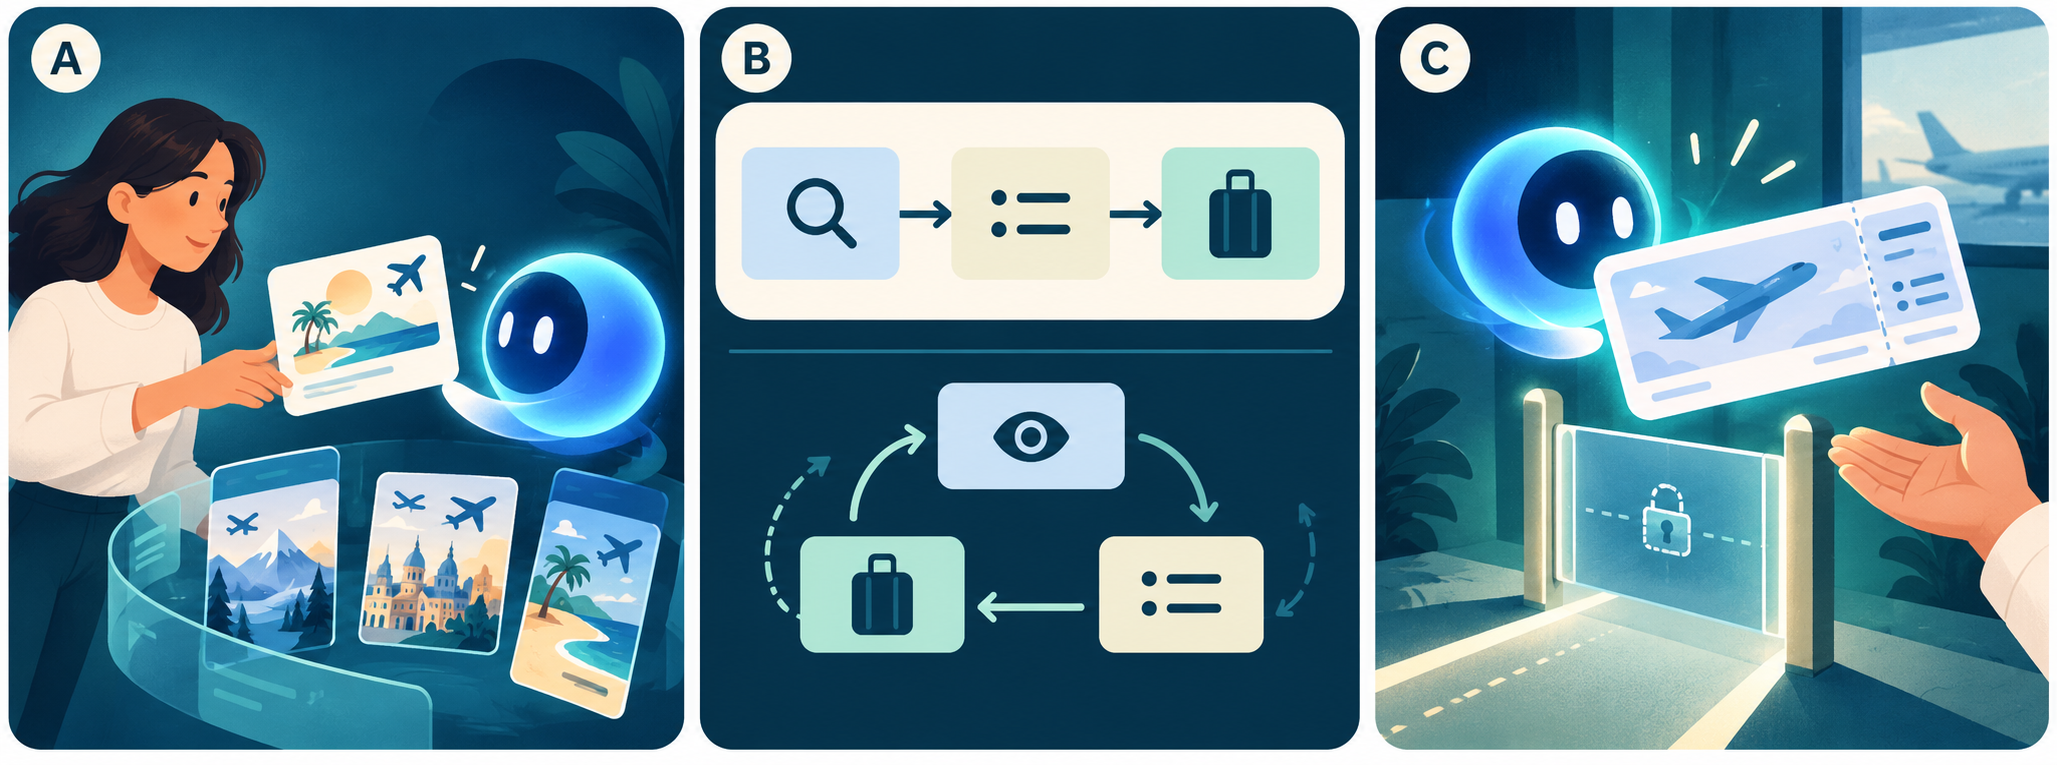
\includegraphics[width=\linewidth,height=0.26\textheight,keepaspectratio]{../assets/figure-8284fa500410.png}\par

{\small 本课重点看 A 区。A 明确委托目标；B 比较固定步骤与观察反馈循环；C 在提交购买前设置人的确认。示意图不代表真实产品界面。}\par

{\footnotesize AI生成教学示意，非实物照片、原始史料或官方架构。生成方式：内置文生图；提示词见仓库 docs/image-prompts.json。}\end{center}

\Needspace{5\baselineskip}\section*{任务的三个要素}

目标描述用户希望得到什么结果，例如获得两套符合时间与预算的往返方案。环境提供任务所需的信息和工具，例如航班查询及日程。完成条件则是可以检查的状态，例如方案包含总价、时间、来源及仍需确认的事项。

Anthropic 的经典文章区分固定编排的工作流与由模型动态决定过程的 Agent；这是一个有用的架构区分，不是全行业唯一术语标准。[S1] 在产品层面，你还要追问：系统有权做什么、无法继续时交给谁，以及结果如何核实。模型能力只是其中一部分。

Google ADK 文档也列出不同类型的 Agent，提示我们框架中的名称不一定等于用户价值。[S5] 不要把“用了多 Agent”写成需求本身；应写清它解决哪一个原本完成不了或完成得很差的步骤。

\Needspace{5\baselineskip}\section*{把完成条件写得可以验收}

不够清楚的条件是“行程合理、体验顺畅”。更可检查的条件是：明确出发与返回日期，列出两套候选，说明价格查询时间，标出退改条件待用户确认，且没有自动付款。

评估还要区分最终结果与执行过程。一个系统可能碰巧选对方案，却读取了不应读取的数据；也可能工具暂时失败，但正确解释了失败并保留进度。Agent 评估材料强调任务与轨迹的关系，本课程据此要求同时观察结果和关键行为。[S3] 这不意味着每条内部思考都应公开，而是用户需要看见与决策相关的状态和证据。

\Needspace{5\baselineskip}\section*{三分钟练习与面试自查}

模拟题：“你会怎样定义旅行助手的第一版？”用四句话回答：服务谁、完成什么、明确不自动做什么、用什么结果验收。

参考：“服务需要快速整理差旅选项的员工；完成符合已知限制的候选对比；购买前由用户确认；以条件满足率、事实正确性和需要返工的比例验收。”这些指标是教学建议，尚无真实测试数据。追问：如果航班查询失败怎么办？合理答案应包括解释、保留已知条件和重试或人工接管，而不是继续编造航班。

\Needspace{5\baselineskip}\section*{复盘与明日连接}

先定义可验证任务，再决定是否需要 Agent。今天的关键不是名词，而是目标、证据与权限能否闭合。明天比较两种实现路线：固定工作流与动态行动，什么时候值得付出更多复杂度？

\Needspace{6\baselineskip}\section*{扩展学习 / Further reading}\small 以下为选读，不计入每日必做时间。\begin{enumerate}[leftmargin=1.6em]

\item [S1] \href{https://www.anthropic.com/engineering/building-effective-agents}{Building effective agents} — 读工作流与 Agent 的区分；用作架构框架，不把旧工具清单当最新。\par Anthropic | 发布：2024-12-19 | 核验：2026-10-08

\item [S2] \href{https://www.anthropic.com/engineering/writing-tools-for-agents}{Writing effective tools for agents} — 关注工具边界、返回结果和评价方法如何影响可用性。\par Anthropic | 发布：2025-09-11 | 核验：2026-10-08

\item [S3] \href{https://www.anthropic.com/engineering/demystifying-evals-for-ai-agents}{Demystifying evals for AI agents} — 理解结果评价与执行轨迹；为后续验收指标课程准备。\par Anthropic | 发布：2026-01-09 | 核验：2026-10-08

\item [S4] \href{https://modelcontextprotocol.io/specification/2025-06-18}{Model Context Protocol specification} — 阅读指定版本的用途和安全原则；不称其为最新版本。\par MCP project | 发布：2025-06-18（指定版本） | 核验：2026-10-08

\item [S5] \href{https://adk.dev/agents/}{Agents in ADK} — 比较 LLM Agent、工作流 Agent 与自定义 Agent 的分类。\par Google ADK | 发布：未标注 | 核验：2026-10-08

\end{enumerate}

\end{document}